\documentclass[a4paper]{article}

\usepackage[utf8]{inputenc}
\usepackage[english]{babel}
\usepackage{graphics}
\usepackage{caption}
\usepackage{subcaption}
\usepackage[demo]{graphicx}
\usepackage{enumitem}
\usepackage{longtable}
\usepackage{listings}
\usepackage{listingsutf8}
\usepackage{framed}
\usepackage{float}
\usepackage{hyperref}
\usepackage{amsmath}

\begin{document}

\begin{titlepage}

\begin{center}
\vspace*{-1in}
\begin{figure}[htb]
\begin{center}

\includegraphics[width=8cm]{logoUZ.png}
\end{center}
\end{figure}

\vspace*{0.3in}

UNIVERSIDAD DE ZARAGOZA \\

\vspace*{0.3in}

\begin{large}
SISTEMAS Y TECNOLOGÍAS WEB\\
\end{large}
\vspace*{0.2in}
\begin{Large}
\textbf{FelinoTweets} \\
\end{Large}
\vspace*{0.3in}
\begin{large}
\end{large}
\vspace*{0.5in}
\rule{80mm}{0.1mm}\\
\vspace*{0.1in}
\begin{large}
Autores: \\
Alejandro Márquez Ferrer (NIP: 566400)\\
Jaime Ruiz-Borau Vizárraga (NIP: 546751)\\
Alejandro Royo Amondarain (NIP: 560285)\\

\end{large}
\end{center}

\end{titlepage}
\tableofcontents

\newpage
\section{Resumen}

	\paragraph{} El trabajo propuesto tiene como objetivo el desarrollo de un sistema que permita gestionar, mediante una interfaz típica de control de acceso de usuarios, una o varias cuentas de \textit{Twitter}.

\section{Propuestas similares - Hootsuite}

	\paragraph{} Se ha analizado principalmente un servicio web similar a la propuesta, \textit{Hootsuite}. Esta herramienta ofrece en su vista principal un panel de control (\textit{dashboard}) para gestionar las cuentas de diferentes redes sociales (\textit{Twitter}, \textit{Facebook}...). Es posible añadir nuevas columnas o eliminarlas para estar al tanto de la mayor cantidad de información posible. 
	
	\paragraph{} Se proporcionan varias versiones de esta aplicación, una gratuita (con funcionalidades limitadas) y otra de pago que ofrece al usuario servicios adicionales como el de realizar informes de estadísticas sobre sus redes sociales.

\section{Arquitectura de alto nivel}
	\paragraph{} A continuación se presenta un diagrama arquitectural de alto nivel con la estructura de la aplicación desarrollada, seguido de una descripción más en detalle de cada una de las partes que la componen:
	\begin{figure}[H]
		\centering
		\includegraphics[width=260px]{diagarq.png}
		\caption{Diagrama arquitectural de alto nivel}
		\label{fig:diagarq}
	\end{figure}
	\newpage
	\subsection{Componentes}
		\begin{itemize}
			\item \textbf{Twitter:} Este componente se encarga de todas las interacciones con Twitter según las solicitudes del Cliente o de otros componentes del servidor. Devuelve y publica tweets y permite realizar retweets o dar "Me gusta".
			\item \textbf{Stats:} Gestiona todas las estadísticas, tanto de usuarios como del administrador del sistema. Se comunica con la base de datos en mLab y con el componente Twitter de FelinoTweets para elaborar las estadísticas.
			\item \textbf{URLs:} Es el componente encargado de acortar urls para publicarlas en los tweets enviados a través de la aplicación. Se comunica con la base de datos para almacenar el usuario que acortó una cierta url, la url acortada y el número de clicks realizados sobre dicha url.
			\item \textbf{Users:} Componente que gestiona los usuarios de la aplicacion de Felino Tweets. Se comunica con la base de datos para obtener información de los usuarios, así como realizar tareas de registro y login.
			\item \textbf{Twitter Accounts:} Por último, este componente gestiona toda la información asociada a cuentas de Twitter, así como sus tokens para poder publicar tweets y recibir información de Twitter.
		\end{itemize}
		\paragraph{} La descripción detallada de cada función del API se encuentra en el apartado \textbf{API}.

\section{Modelo de datos}

	\paragraph{} Se han definido varias colecciones para almacenar la información de los disintos usuarios de la aplicación, de sus cuentas de twitter, de los enlaces a acortar o para almacenar estadísticas que proporcionan a los usuarios, ya sean administradores o usuarios normales una retroalimentación de su interacción con la aplicación. A continuación se describen todas las colecciones utilizadas:
	
	\begin{itemize}
	\item \textbf{hashtag}: contiene la información almacenada sobre cada \textit{hashtag}.
		
		\begin{itemize}
		\item user\_id : String,
		\item account\_id : String,
		\item hashtag : String
		\end{itemize}
		
	\item \textbf{registrations}: almacena la información relativa a los diferentes eventos de acceso que pueden tener lugar: \textit{alta}, \textit{baja} y \textit{acceso}. Asociada a cada evento se guarda también la fecha, de esta forma se puede utilizar esta colección para crear estadísticas al respecto.
		
		\begin{itemize}
		\item type : String,
		\item date : Date
		\end{itemize}
	 
	\item \textbf{scheduled\_tweets}: contiene toda la información necesaria para representar un \textit{tweet}.
	
		\begin{itemize}
		\item user\_id : String,
		\item account\_id : String,
		\item date : Date,
		\item text : String
		\end{itemize}
	
	\item \textbf{twitter\_accounts}: guarda la información relativa a la asociación entre una cuenta de \textit{twitter} y una cuenta de usuario de la aplicación, así como los tokens necesarios para comunicarse con el \textbf{API} de \textit{Twitter}.
	
		\begin{itemize}
		\item account\_id : String,
		\item token : String,
		\item token\_secret : String,
		\item profile\_name : String,
		\item photo\_url : String,
		\item description : String,
		\end{itemize}
	
	\item \textbf{url}: contiene la asociación entre \textit{urls} acortadas y \textit{urls} originales para poder realizar la redirección.
	
		\begin{itemize}
		\item short\_url : String,
		\item long\_url : String,
		\item user\_id : String,
		\item clicks : Number
		\end{itemize}
	
	\item \textbf{user}: almacena toda la información relativa a un usuario de la aplicación. Se guardan tanto datos personales como fechas de acceso y registro o número total de tweets enviado (representan la suma de tweets enviados por todas las cuentas de \textit{twitter} asociadas a dicho usuario).
	
		\begin{itemize}
		\item admin : Boolean,
		\item email : String,
		\item password : String,
		\item first\_name : String,
		\item last\_name : String,
		\item registration\_date : Date,
		\item last\_access\_date : Date,
		\item n\_tweets : Number		
		\end{itemize}
	
	\end{itemize}

\newpage
\section{API REST}

	\paragraph{} En este apartado se recogen todos los endpoints de cada componente del API desarrollados, junto a una descripción de lo que hace, sus parámetros y ejemplos de uso.
	
	\subsection{API del componente Twitter}
	\begin{itemize}
		\item \textbf{GET /twitter/tweet\_account:} Devuelve una cuenta de twitter asociada al usuario de FelinoTweets que recibe por parámetro, la cual tambien está referenciada en el body de la petición. Los parámetros que admite son el id del usuario de FelinoTweets, ya sea a través del body o a través de la cookie del navegador, y el nombre de la cuenta de twitter.
		
		\item \textbf{GET /twitter/tweetline:} Devuelve la timeline de una cuenta de twitter. Los parámetros que admite son el id del usuario de FelinoTweets, ya sea a través del body o a través de la cookie del navegador, y el nombre de la cuenta de twitter.
		
		\item \textbf{GET /twitter/home:} Devuelve el home de una cuenta de twitter. Los parámetros que admite son el id del usuario de FelinoTweets, ya sea a través del body o a través de la cookie del navegador, y el nombre de la cuenta de twitter.
		
		\item \textbf{GET /twitter/mentions:} Devuelve las menciones de una cuenta de twitter. Los parámetros que admite son el id del usuario de FelinoTweets, ya sea a través del body o a través de la cookie del navegador, y el nombre de la cuenta de twitter.
		
		\item \textbf{GET /twitter/md:} Devuelve los mensajes directos de una cuenta de twitter. Los parámetros que admite son el id del usuario de FelinoTweets, ya sea a través del body o a través de la cookie del navegador, y el nombre de la cuenta de twitter.
		
		\item \textbf{POST /twitter/tweet:} Postea un nuevo tweet dada una cuenta de twitter pasada por parámetro. Los parámetros que admite son el id del usuario de FelinoTweets, ya sea a través del body o a través de la cookie del navegador, y el nombre de la cuenta de twitter.
		
		\item \textbf{POST /twitter/md:} Envía un nuevo mensaje directo dada una cuenta de twitter pasada por parámetro. Los parámetros que admite son el id del usuario de FelinoTweets, ya sea a través del body o a través de la cookie del navegador, y el nombre de la cuenta de twitter.
		
		\item \textbf{POST /twitter/retweet:} Realiza un retweet dada una cuenta de twitter pasada por parámetro y un tweet de origen. Los parámetros que admite son el id del usuario de FelinoTweets, ya sea a través del body o a través de la cookie del navegador, el nombre de la cuenta de twitter y el tweet al que se realiza el retweet.
		\newpage
		\item \textbf{POST /twitter/unretweet:} Deshace un retweet dada una cuenta de twitter pasada por parámetro y un tweet de origen. Los parámetros que admite son el id del usuario de FelinoTweets, ya sea a través del body o a través de la cookie del navegador, el nombre de la cuenta de twitter y el tweet al que se quita el retweet.
		
		\item \textbf{POST /twitter/fav:} Realiza un "me gusta" dada una cuenta de twitter pasada por parámetro y un tweet de origen. Los parámetros que admite son el id del usuario de FelinoTweets, ya sea a través del body o a través de la cookie del navegador, el nombre de la cuenta de twitter y el tweet al que se realiza el "me gusta".
		
		\item \textbf{POST /twitter/unfav:} Quita un "me gusta" dada una cuenta de twitter pasada por parámetro y un tweet de origen. Los parámetros que admite son el id del usuario de FelinoTweets, ya sea a través del body o a través de la cookie del navegador, el nombre de la cuenta de twitter y el tweet al que se quita el "me gusta".
		
		\item \textbf{GET /twitter/auth:} Realiza una llamada al middleware Passport.js que se encarga de gestionar la interacción con Twitter para autorizar a la aplicación FelinoTweets a que utilice una determinada cuenta de Twitter. Realiza una redirección al servicio de autorización de Twitter.
		
		\item \textbf{GET /twitter/auth/callback:} Es el endpoint al que accede el middleware Passport.js cuando retorna de la llamada a Twitter para autorizar una cuenta de twitter. Trae de vuelta los tokens que permiten utilizar una cuenta de Twitter desde una aplicación externa que no sea Twitter.
	\end{itemize}
	
	\subsection{API del componente Stats}
	\begin{itemize}
		\item \textbf{GET /stats/registrations/:days:} 
		\item \textbf{GET /stats/registrations/:type/:days:} 
		\item \textbf{POST /stats/registrations/:} 
		\item \textbf{GET /stats/ranking/tweets/:limit:} 
		\item \textbf{GET /stats/ranking/accounts/:limit:} 
		\item \textbf{GET /stats/activeUsers/:days:} 
		\item \textbf{GET /stats/mentions/:id:} 
		\item \textbf{GET /stats/multimedia/:id:}
		\item \textbf{GET /stats/hashtags/:id:} 
		\item \textbf{GET /stats/retweets/:id:}
		\item \textbf{GET /stats/tweets/:id:}
		\item \textbf{GET /stats/ranking/mentions/:limit/:id:}  
	\end{itemize}
	\subsection{API del componente URLs}
	\begin{itemize}
		\item \textbf{GET /url:} Devuelve una lista con todas las URLs acortadas de la base de datos. No admite ningún parámetro.
		\item \textbf{GET /url/:short\_url:} Redirige la petición a la url original que fue acortada. El único parámetro que admite es el identificador de la url acortada.
		\item \textbf{POST /url/:} Provee una url para su acortamiento y posterior almacenamiento en la base de datos junto con los datos del usuario que solicita el acortamiento. Admite como parámetros la url larga para acortar y el id del usuario que solicita su acortamiento. Dichos parámetros deben ir en el cuerpo de la petición.
		\item \textbf{DELETE /url/:} Elimina todas las urls acortadas almacenadas en la base de datos. No admite parámetros.
		\item \textbf{DELETE /url/:short\_url:} Elimina la url acortada especificada por el parámetro short\_url de la base de datos. El único parámetro que admite es la url acortada.
	\end{itemize}
	
	\subsection{API del componente Users}
	
	\subsection{API del componente Twitter accounts}
\section{Analíticas}

	\paragraph{} Se ha desarrollado un servicio de analíticas que ofrece datos acerca del comportamiento del conjunto de usuarios de la aplicación para un usuario de tipo administrador. Por otro lado, el mismo servicio ofrece estadísticas acerca de las cuentas de \textit{Twitter} asociadas con un usuario.
	
	\subsection{Analíticas de administrador}
	
		\paragraph{} El objetivo de estas estadísticas es el de dar al administrador una visión del modo en que sus usuarios utilizan la aplicación. A continuación se muestran las gráficas que puede visualizar el administrador del sistema:
		
			\begin{figure}[H]
				\centering
				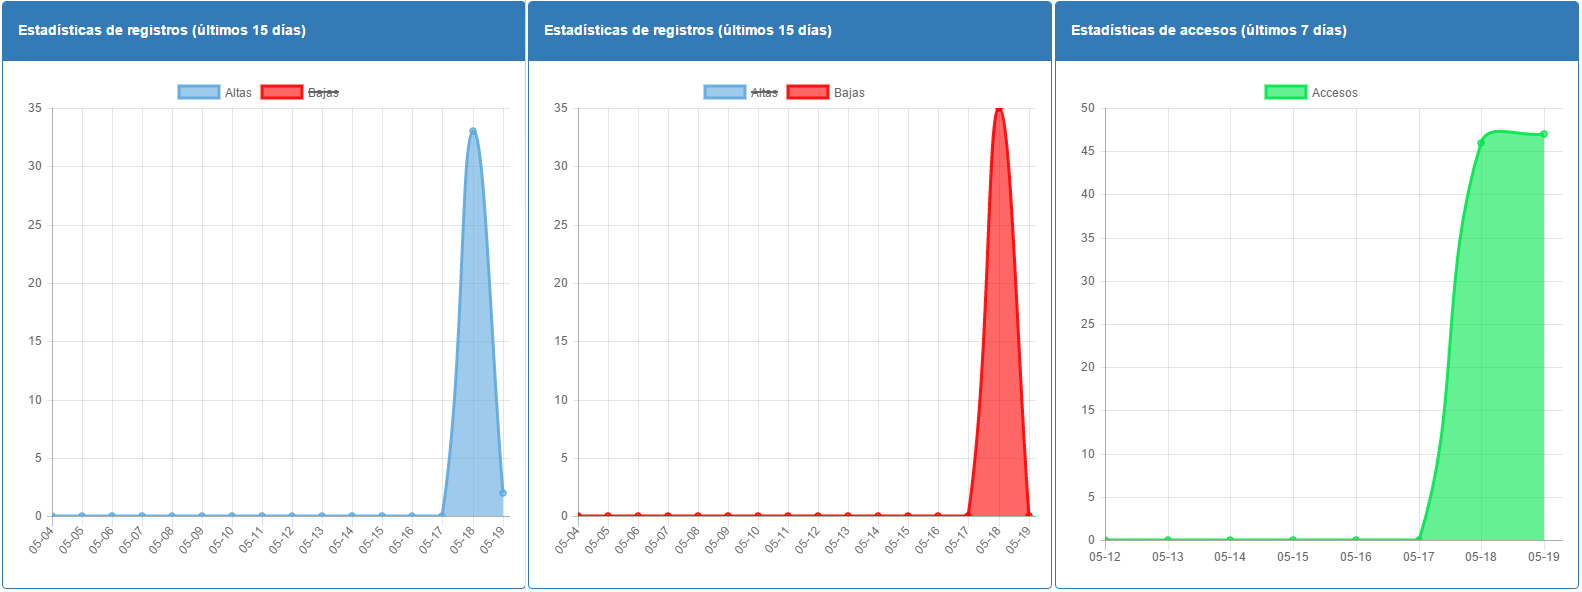
\includegraphics[width=1\linewidth]{img/altas-bajas-accesos}
				\caption{Registros, cuentas borradas en la aplicación en los útlimos 15 días y accesos de los usuarios (no únicos) a la apliación en los últimos 7 días.}
				\label{fig:altas-bajas-accesos}
			\end{figure}
			
			\begin{figure}[H]
				\centering
				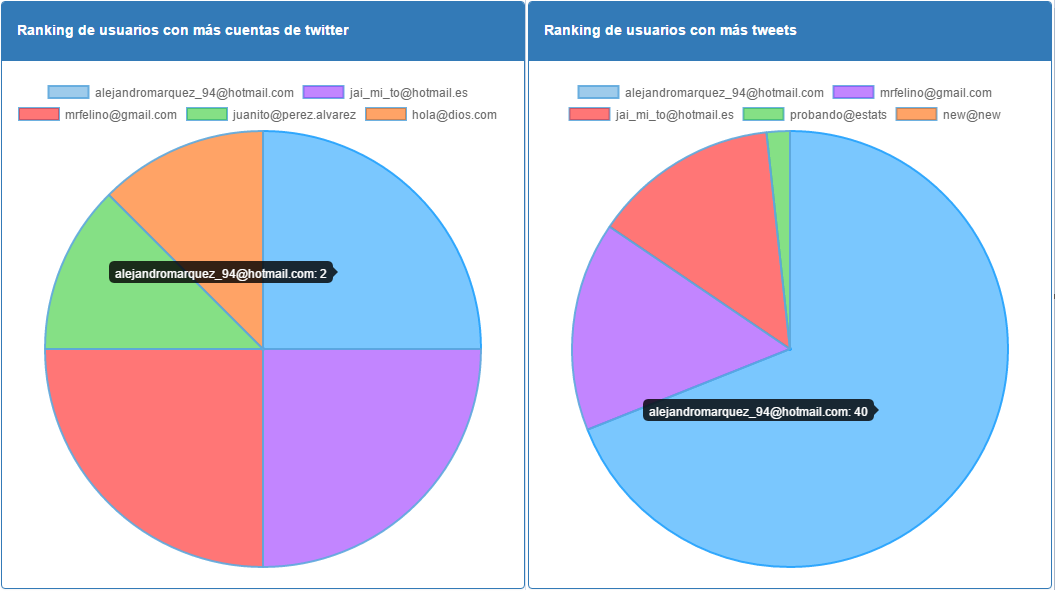
\includegraphics[width=1\linewidth]{img/rankingsAdmin}
				\caption{Ranking de cuentas con mayor número de tweets enviados (izquierda) y ranking de cuentas de la aplicación con mayor número de cuentas de twitter asociadas cada una (derecha).}
				\label{fig:rankingsAdmin}
			\end{figure}
	
	\subsection{Analíticas de usuario} 

		\paragraph{} El interés de estas gráficas para el usuario reside en informarle de la diferente repercursión que tienen sus disintas cuentas de \textit{Twitter} asociadas. 
		
			\begin{figure}[H]
				\centering
				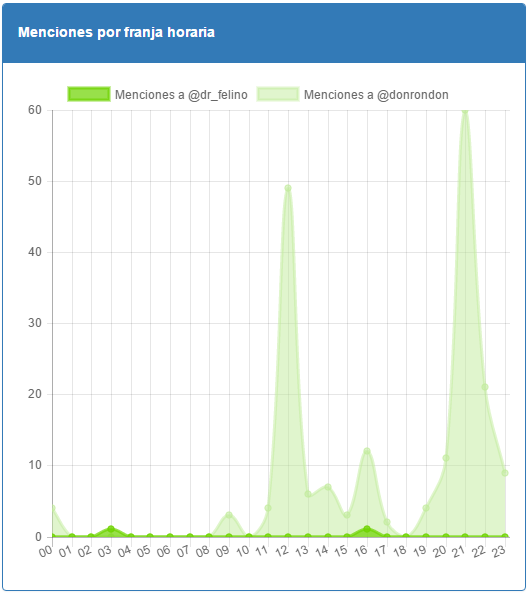
\includegraphics[width=0.6\linewidth]{img/mencionesHoras}
				\caption{Número de menciones con cada cuenta del usuario distribuidas por franja horaria.}
				\label{fig:mencionesHoras}
			\end{figure}
			
			\begin{figure}[H]
				\centering
				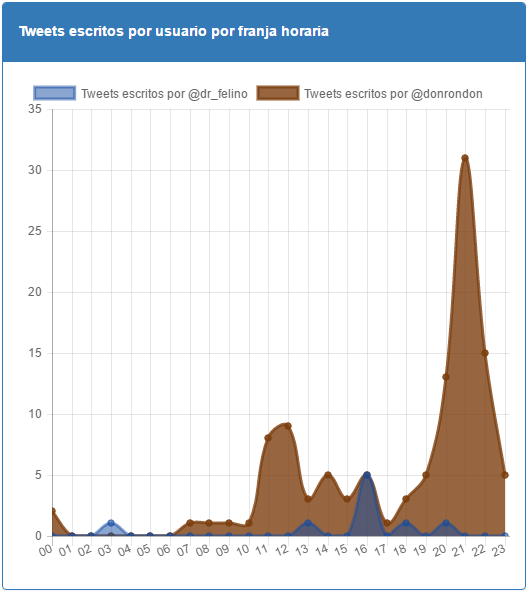
\includegraphics[width=0.6\linewidth]{img/tweetsHoras}
				\caption{Número de tweets enviados con cada cuenta del usuario distribuidos por franja horaria.}
				\label{fig:tweetsHoras}
			\end{figure}
			
			\begin{figure}[H]
				\centering
				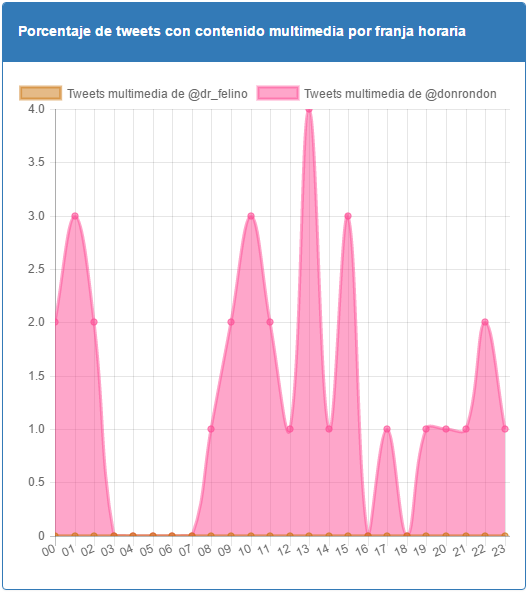
\includegraphics[width=0.6\linewidth]{img/tweetsMultimedia}
				\caption{Porcentaje de tweets con contenido multimedia con cada cuenta del usuario y distribuidos por franja horaria.}
				\label{fig:tweetsMultimedia}
			\end{figure}
			
			\begin{figure}[H]
				\centering
				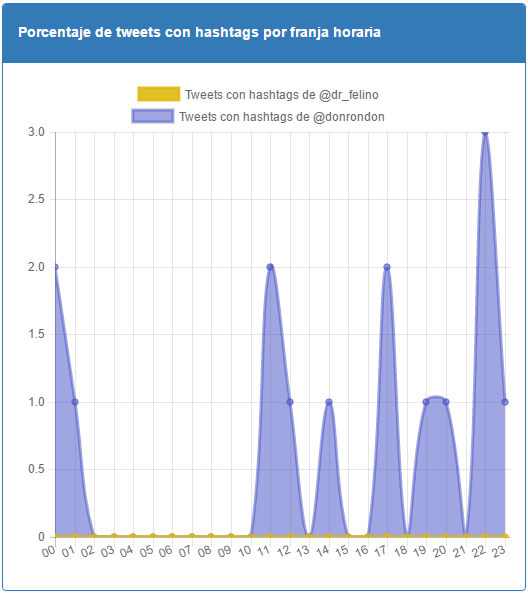
\includegraphics[width=0.6\linewidth]{img/hashtagsHoras}
				\caption{Porcentaje de tweets con contenido multimedia con cada cuenta del usuario y distribuidos por franja horaria.}
				\label{fig:hashtagsHoras}
			\end{figure}
			
			\begin{figure}[H]
				\centering
				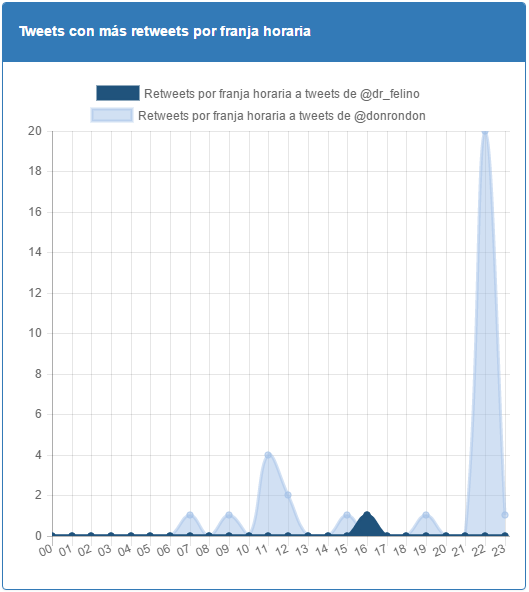
\includegraphics[width=0.6\linewidth]{img/retweetsHoras}
				\caption{Cantidad de retweets realizados sobre tweets escritos en determinada franja horaria para cada cuenta del usuario.}
				\label{fig:retweetsHoras}
			\end{figure}
			
			\begin{figure}[H]
				\centering
				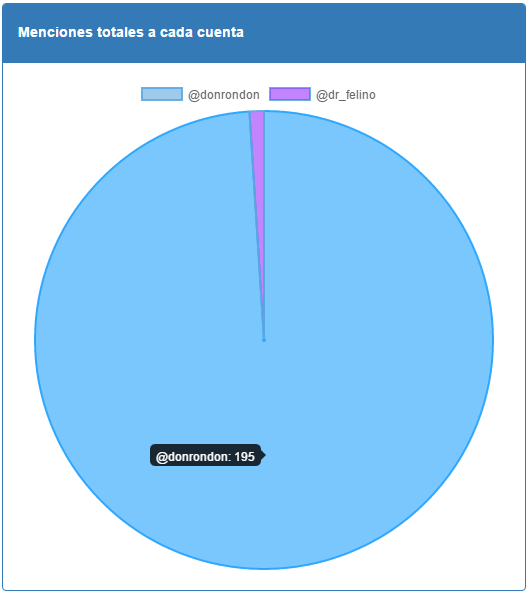
\includegraphics[width=0.6\linewidth]{img/mencionesCuentas}
				\caption{Cantidad de menciones para cada cuenta del usuario (representa impacto de cada cuenta de twitter en su entorno.)}
				\label{fig:mencionesCuentas}
			\end{figure}

\section{Implementación}

	\paragraph{} Para el desarrollo de la aplicación web propuesta se ha hecho uso del conjunto de tecnologías denominado como \textbf{\textit{MEAN Stack}} (\textit{MongoDB}, \textit{Express}, \textit{AngularJS}, \textit{Node}). Para el desarrollo del \textit{front-end} se han usado \textit{AngularJS + Bootstrap} y para el desarrollo del \textit{back-end} se han utilizado \textit{MongoDB} para la base de datos y \textit{Express} y \textit{Node} para el desarrollo del servidor, lo cual asegura escalabilidad.

	\subsection{Desarrollo de \textit{front-end}}
	
		\paragraph{} Se ha optado por realizar la gestión de enrutamiento mediante \textit{AngularJS} aprovechando las facilidades que proporciona en la implementación de un modelo vista-controlador.
		
		\paragraph{} En primer lugar, se ha definido en un fichero \textbf{public/app.js} el conjunto de estados (vistas) en los que se puede encontrar la aplicación de forma, que es el que se encarga de redirigir correctamente cualquier petición de cambio de estado. Éste módulo también se encarga de asignar a cada estado una vista \textit{.html} con un controlador \textit{.js}.
	
		\paragraph{} Cada controlador gestiona de forma dinámica su vista asociada. En el caso de invocar a un \textit{API} externa se comunica con el módulo principal de los controladores (\textit{public/app.js}) y es éste el único que realiza las peticiones \textbf{.http}. Así se consige modular el código, de forma que es más fácil su depuración.
	
		\paragraph{} Por último, todas las vistas (\textit{.html}) utilizan \textit{Bootstrap} para asegurar que la aplicación se pueda visualizar correctamente en dispositivos con pantallas de distintos tamaños.
		
	\subsection{Desarrollo de \textit{back-end}}
	
		\paragraph{} Dado que es el \textit{front-end} el que se encarga de enrutar las peticiones, la función del servidor en este aspecto es la de para cualquier petición que reciba redirigir al \textit{front-end}. De esta forma el servidor se limita a proporcionar los distintos servicios web propuestos (\textit{control de usuarios}, \textit{acortador de URLs} y servicio de \textit{estadísticas}).
		
		\paragraph{} El servidor se ha implementado con \textit{node.js}, de esta forma se asegura una buena escalabilidad de la aplicación. En este sentido la gestión de la base de datos mediante \textit{Mongoose} también ayuda a mejorar esta característica.
		
\section{Modelo de navegación}

\section{Despliegue del sistema (instrucciones)}
\paragraph{}Para desplegar el sistema se hace uso de Heroku, una plataforma que permite montar la aplicación de manera gratuita (con limitaciones, pero para el alcance del proyecto es más que suficiente) de una manera fácil y sencilla. Está configurado de tal manera que se despliegue automáticamente a partir del repositorio de GitHub de \href{https://github.com/FelinoSoft/FelinoTweets}{FelinoTweets}. De esta forma, la aplicación se actualizará con cada commit realizado sobre la branch principal del repositorio.
\paragraph{}La aplicación contiene un fichero de configuración, siguiendo la ruta a partir de la raíz \textit{/confi/config.json}. En él hay que definir los siguientes campos;
\begin{itemize}
\item \textbf{domain}: el dominio de la aplicación.
\item \textbf{port}: el puerto en el que escuchará la aplicación.
\item \textbf{consumerKey}: la clave de consumidor de Twitter, para realizar las operaciones con el API de Twitter (esto se explicará más adelante).
\item \textbf{consumerSecret}: la clave secreta de Twitter, que junto con la anterior, permite autentificarse como una App de Twitter.
\item \textbf{databaseAddress}: dirección de la base de datos sobre la que se realizarán las consultas y almacenarán los datos de la aplicación.
\item \textbf{API}: ruta de la API de la aplicación, sobre la que se situarán los endpoints.
\end{itemize}

\paragraph{}Los apartados \textit{consumerKey} y \textit{consumerSecret} contienen las claves de la aplicación de Twitter. Para poder realizar operaciones al API de Twitter, es necesario haber creado antes una Twitter App, en su página oficial, que permitirá a los usuarios autentificarse o loguearse a Twitter a través de la aplicación, y de esta manera realizar en su lugar operaciones (como postear tweets, hacer búsquedas...). Estas dos claves sirven para identificarse de una manera segura como aplicación de Twitter, y no deben ser ni compartidas ni públicas.

\paragraph{}La base de datos de la aplicación está proporcionada por \href{https://mlab.com/}{mLab}, un servicio de base de datos \textit{Database-as-a-Service} para MongoDb. Al igual que Heroku, tiene ciertas limitaciones, pero sus funcionalidades son más que suficientes para el proyecto.

\paragraph{}Por último, para terminar de desplegar el sistema y dejarlo listo para funcionar, hay que añadir un usuario que actuará como administrador, y de esta manera, podrá realizar operaciones sobre los usuarios y sus cuentas.

\section{Validación (test, pruebas realizadas)}
\paragraph{}Para probar el correcto funcionamiento de la aplicación, se han ido probando mediante Postman todas las operaciones disponibles sobre los endpoints de las APIs, obteniendo el comportamiento deseado. Finalmente, se ha realizado un recorrido por toda la aplicación, que se detalla a continuación:
\begin{itemize}
	\item \textbf{Paso: }Registro de un usuario. \textbf{Resultado: }
\end{itemize}

\section{Análisis de problemas}

	\paragraph{} Dado que es la primera vez que el equipo afronta un desarrollo web de estas características, se ha encontrado como princpal dificultad el aprendizaje de las nuevas tecnologías con las que se requería realizar el proyecto.
	
	\paragraph{} Por otro lado, ha resultado complicado plantear la estructura del código a implementar en cuanto a cómo debía gestionarse el enrutamiento y cual es la mejor estrategia para organizar los directorios de una aplicación con características como múltiples vistas y de las dimensiones que tiene la aplicación propuesta. Todas estas cuestiones cobran mayor importancia al ser la primera vez que se afrontan.

\section{Distribución de tiempos}
	\subsection{Diagrama de Gannt}
	\subsection{Horas de esfuerzo del equipo y por separado en tareas}

\section{Conclusiones}
	\subsection{Conclusiones del proyecto}
	
		\paragraph{} La realización de este proyecto ha generado como resultado una aplicación web \textit{responsive} que permite al usuario gestionar cuentas de \textit{Twitter} así como ver estadísticas de las mismas.
		
		\paragraph{} Durante el desarrollo del proyecto se ha trabajo con un \textit{API} externa que es la de \textit{Twitter}, lo cual ha resultado útil a la hora de entender cómo se comunican las aplicaciones web actualmente. 
	
	\subsection{Valoración personal del grupo}
	
		\paragraph{} El proyecto ha ayudado principalmente a comprender el funcionamiento de un servicio web y de los canales de comunicación así como tecnologías mas usadas actualmente, lo cual puede servir de ayuda para futuros desarrollos.
	
		\paragraph{} El desarrollo con nuevas tecnologías ha sido desafiante pero al mismo tiempo gratificante, ya que se obtienen resultados simples con rapidez. El equipo ha quedado satisfecho con el resultado conseguido aunque se considera que el tiempo disponible para realizarlo ha sido muy ajustado.
		
	\subsection{Valoración personal de cada miembro}
	
\newpage
\begin{thebibliography}{99} 
\bibitem{paraQueSirve} \textbf{Title} - Consulted in XXXXX aaaa. [\url{link}]

\end{thebibliography}

\end{document}